\subsection{Observability in \abstraction{}}
\label{rasc:sec:rasc}

The goals of action progress updates and failure detection (\Cref{rasc:tab:properties}) can be served via a mechanism that {\it periodically polls} the device for its current state. This polling needs to (i) satisfy user-specified tolerances for detecting failures, (ii) balance detection latency vs. device/network load, and (iii) adapt to evolving action time distributions (i.e., wrong estimates). 

\begin{figure}[th]
    \centering
    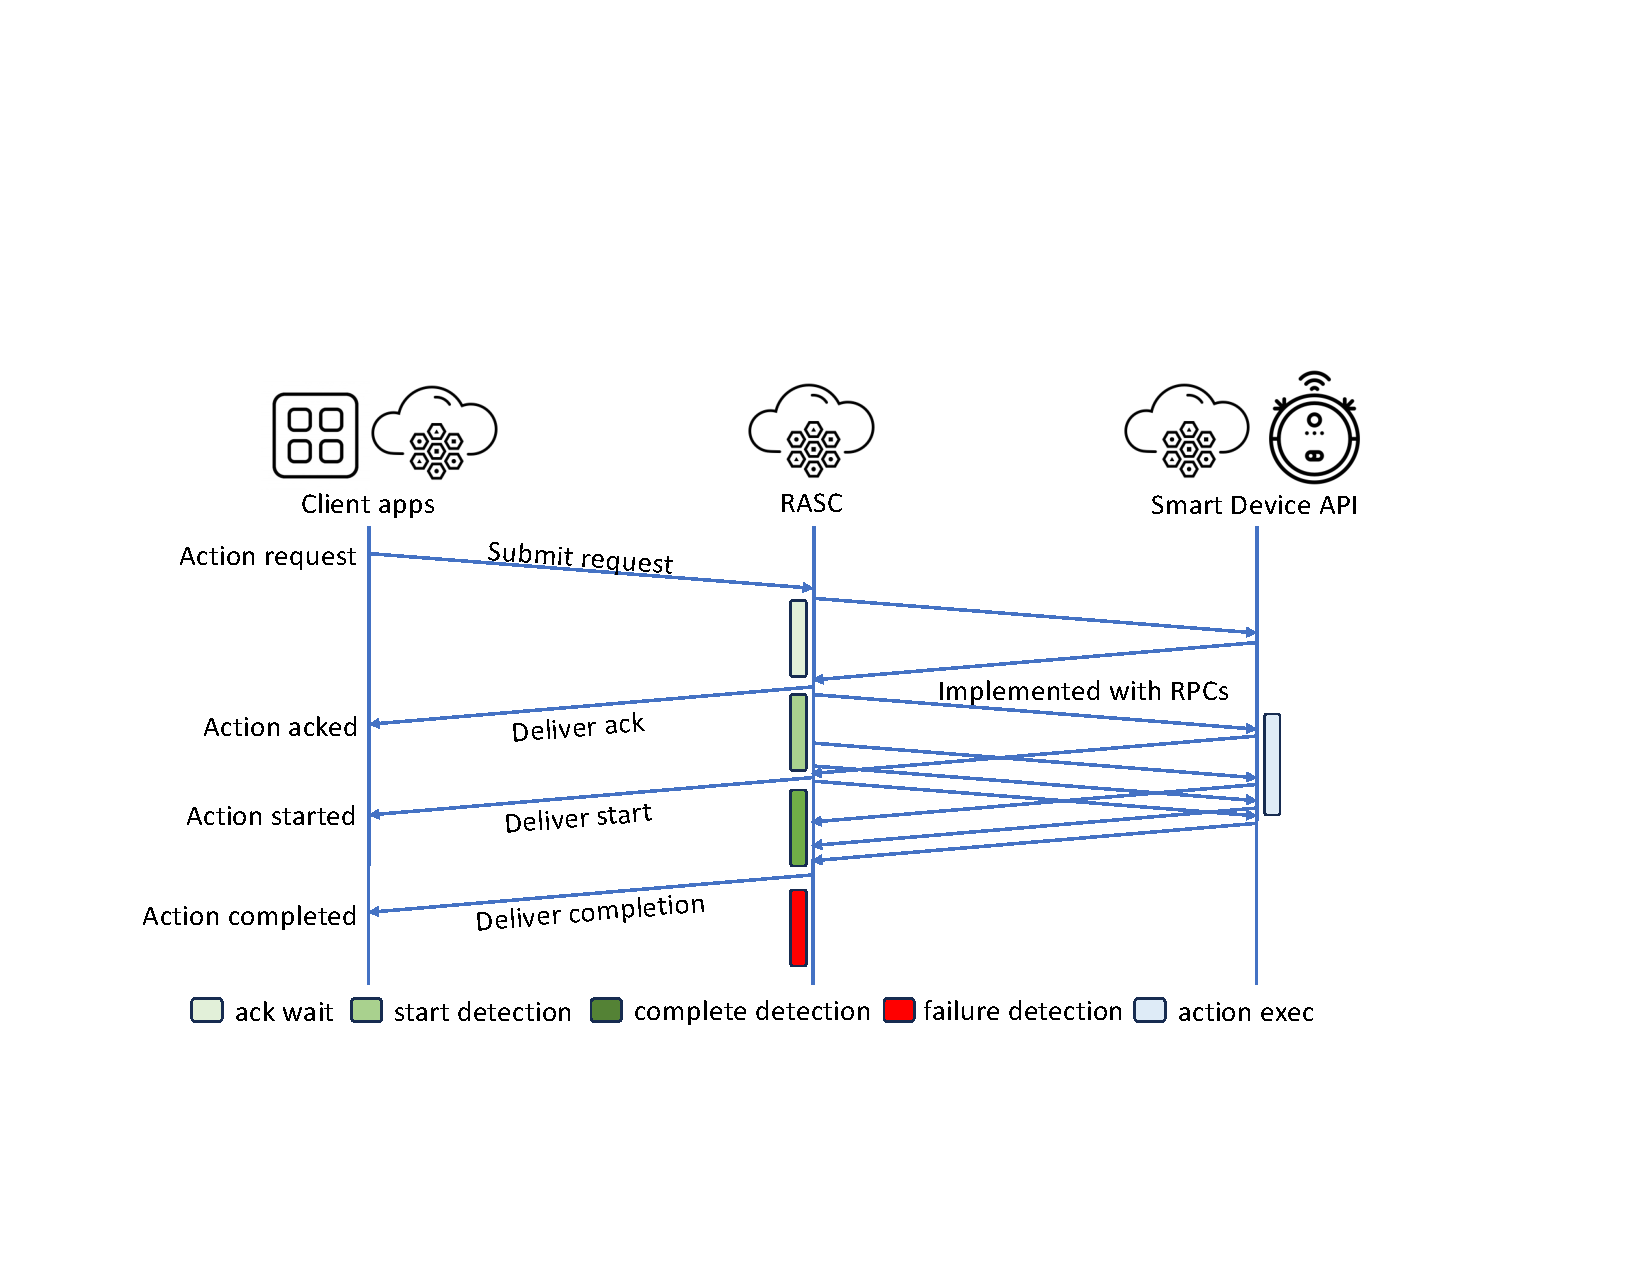
\includegraphics[width=0.9\linewidth,alt={Diagram of the RASC abstraction layered over RPCs. RASC provides three responses: acknowledgment, start, completion, and/or failure. The frequent RPCs shown on the right are the adaptive polls that RASC issues in the background to track an action's progress.}]{RASC/figures/design/RASC abstraction.pdf}
    \caption{\bf \small \abstraction{} over RPCs. {\it Frequent RPCs on right are polls.}
    }
    \medskip
    \label{rasc:fig:rasc_design}
\end{figure}

\noindent \textbf{Lifetime of an Action.} \Cref{rasc:fig:rasc_design} shows how 
\abs{} runs backward-compatibly over the RPC layer.  
For a given action, \sysname{} cycles through 
four states (or stages or phases, which we use interchangeably): 
{\it ack wait, start detection, complete detection}, and {\it failure detection}.
When the action is requested, \sysname{} is in the {\it ack wait} state. Immediately after the hub receives an ack (that the device or its web service has received the request), \sysname{} enters the {\it start detection} phase, wherein it starts tracking the state of the device (described in \Cref{rasc:sec:adaptive-polling-strategy}).
Alternatively, if the IoT device is unresponsive, then \sysname{} enters the {\it failure detection state}.
The user specifies a {\bf tolerance threshold} $Q_w$ in seconds (maximum time between a state change and its detection), and \sysname{} needs to meet it. 


If the action is short, 
the action completion target state might be detected alongside or soon after the start.
So during the start detection state, \sysname{} also checks if either of the start or completion states is already matched, and if so, short-circuits to the complete detection state. 

In IoT settings, it is impossible to distinguish a failed device from one that is not executing actions at all. So \sysname{} detects the failure of {\it actions}, but does not declare a device as being failed. \sysname{} reports failures to the user (who may take subsequent actions like restarting the device).

\begin{figure}[h]
    \centering
    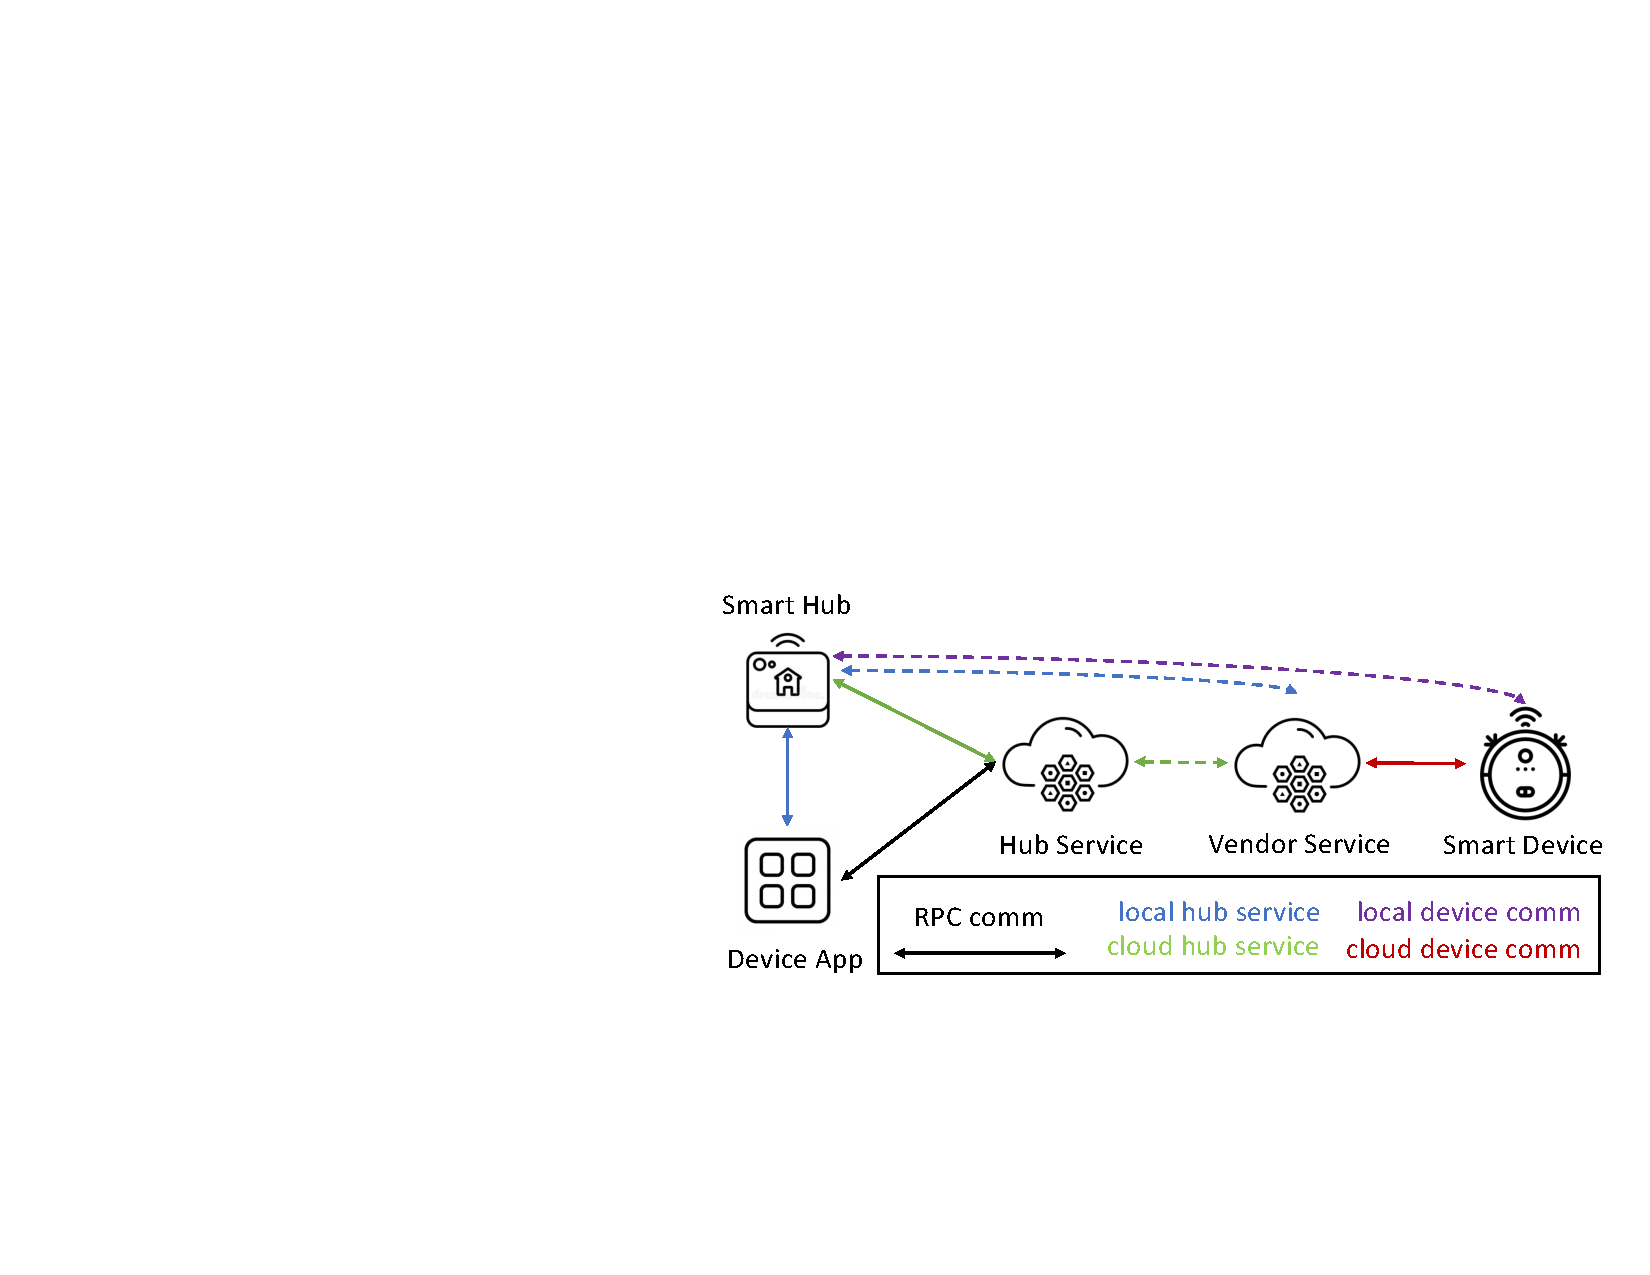
\includegraphics[width=0.65\linewidth,alt={Diagram of communication between a smart device and a client app. Each arrowed line is an RPC in today's stacks; the dashed lines are the ones this work replaces with the new RASC abstraction. A client device app or smart hub communicates either directly with the device (hub-to-device) or via a vendor cloud service (hub-to-cloud-to-device). The device app may also first communicate with the smart hub.}]{RASC/figures/intro/smart space setup.pdf}
    \caption{\bf \small Communication between a smart device and a client app. {\it Each arrowed line is an RPC in today's stacks. This paper replaces dashed lines with the new \abs{} abstraction.}
    }
    \medskip
    \label{rasc:fig:iot setup}
\end{figure}

\noindent \textbf{IoT Architecture.}
\Cref{rasc:fig:iot setup} shows how  \abs{} is built atop today's RPC mechanisms. 
\abs{} interfaces
user devices and applications 
(running on the Hub Service, e.g., Alexa, Google Home), with 
the device or its vendor service  (e.g., web microservices run by the device vendor, e.g., Philips Hue, GE Sync, etc.). 
In \Cref{rasc:fig:iot setup}, \abs{} replaces only those RPCs at dashed arrows, while solid arrow RPCs remain. 
Every path from the hub/user device to the IoT device contains exactly one \abs{} call. 
{\abs{} needs to modify only the cloud services and hubs but not the device or vendor services.} 

\subsubsection{Adaptive Polling Strategy}
\label{rasc:sec:adaptive-polling-strategy}

Both progress updates and failure detection require \emph{polling} that is (i) efficient (few messages) and (ii) responsive (detects changes quickly).
For \emph{push} devices (\Cref{rasc:sec:model}), this is straightforward---the device or vendor notifies the hub, which relays to \sysname{}. 
The challenge is \emph{pull}-only devices.
Polling too aggressively (e.g., every 500\,ms) can overload devices and the network; polling too sparsely increases detection latency. 
Key questions arise: {\it What polling frequency is appropriate? Should polling become more frequent as it progresses?} 

\noindent \textbf{\underline{Problem Statement}.}
We seek to minimize \emph{detection time}: the gap between the action state change on a device and \sysname's next poll.
Inputs are: (i) the {\bf historical state-change time distribution} \(p(t)\) for a (device, action) pair---\texttt{dist.pdf(t)}, (ii) a {\bf state change time bound} $U$---\texttt{dist.ppf(0.99)}\footnote{Percent point function (inverse cdf); \(\texttt{ppf}(y)\) returns the value with cdf \(y\).} which may occasionally be exceeded, and (iii) a poll \textbf{budget} \(k\) representing how many total polls are allowed for a given action (representing allowable bandwidth).
We must 
select \(k\) poll timepoints in \((0,U]\) that minimize expected detection time.

\noindent \textbf{Solution.}
Let the $k$ poll times be $L_i, i=1,...,k$. Then the expected detection time $Q$ can be formulated as:
{\small
\begin{align}
Q &= \int_{0}^{L_1} (L_1-t)p(t)\,dt 
   + \int_{L_1}^{L_2} (L_2-t)p(t)\,dt + \cdots \notag \\ 
  &+ \int_{L_{k-1}}^{L_k} (L_k-t)p(t)\,dt \tag{1} \\
Q &= \sum_{i=1}^{k} L_i \int_{L_{i-1}}^{L_i} p(t)\, dt
   - \int_{0}^{L_k} t\,p(t)\, dt \tag{2} \label{rasc:eq:Q}
\end{align}
}

Here, each term $i$ represents the expected detection time of $L_i$ if the change happens before $L_i$ and after $L_{i-1}$. The highest ${L_k}$ is always equal to $U$.
The second term here is the average of $p(t)$, and thus a constant we can ignore to optimize $Q$.

\begin{theorem}[Adaptive Poll Placement with Fixed Budget $k$]
Given a time distribution $p(t)$ on $(0,U]$, a poll budget $k$, and a terminal tolerance $\varepsilon>0$,
polls
$0<{L_1^{\!*}}<\cdots<L_{k-1}^{\!*}<L_k^{\!*}$
that \underline{minimize 
expected detection time} $Q$ and satisfy $\lvert L_k^{\!*}-U\rvert\le\varepsilon$ are given by the following recurrent relation:
{%\small
\[
L_i^{\!*} =
\begin{cases} 
\frac{1}{p(L_{i-1}^{\!*})} \cdot \int_{L_{i-2}^{\!*}}^{L_{i-1}^{\!*}} p(t)\, dt + L_{i-1}^{\!*} & \text{for } i \in \{2,\dots,k\}, \\
\text{value } \in (0,U] & \text{for } i=1
\end{cases} {\tag{\small 3}} \label{rasc:eq:recurrence}
\]
}
\end{theorem}

\begin{proof}
Per \eqref{rasc:eq:Q}, only the $i$-th and $(i+1)$-th terms of $Q$ depend on $L_i$:
\[
A_i=\int_{L_{i-1}}^{L_i} (L_i-t)\,p(t)\,dt,\qquad
A_{i+1}=\int_{L_i}^{L_{i+1}} (L_{i+1}-t)\,p(t)\,dt.
\]
By Leibniz's rule,
\[
\frac{\partial A_i}{\partial L_i}
= (L_i{-}L_i)p(L_i) + \int_{L_{i-1}}^{L_i} \frac{\partial}{\partial L_i}\big[(L_i{-}t)p(t)\big]\,dt
= \int_{L_{i-1}}^{L_i} p(t)\,dt,
\]
and
\[
\frac{\partial A_{i+1}}{\partial L_i}
= -\,(L_{i+1}-L_i)\,p(L_i).
\]
The first-order optimality condition $\partial Q/\partial L_i=0$ gives
\[
\int_{L_{i-1}}^{L_i} p(t)\,dt \;-\; (L_{i+1}-L_i)\,p(L_i) \;=\;0,
\]
which rearranges to the recurrence relation \eqref{rasc:eq:recurrence}.
Under $p>0$ and continuity, 
these conditions determine a unique sequence once $L_1$ is fixed.
We fix $L_1\in(0,U)$ and generate $L_2,\dots,L_k$ via \eqref{rasc:eq:recurrence}.
Then $L_k(L_1)$ is strictly increasing in $L_1$.
Hence, there exists a unique $L_1^*\in(0,U)$ such that the generated sequence satisfies
$L_k^*=U$.
\end{proof}

\begin{algorithm}[t!]
    \caption{\bf Adaptive Polling Algorithm}
    \label{rasc:algo:adaptive-polling-algorithm}
    \footnotesize
    \algtext*{EndIf} % hide EndIf but keep block structure
    \algtext*{EndElse} % same for Else
    \algtext*{EndFor} % same for For
    \begin{algorithmic}[1]
        \Procedure{FindPolls}{dist, $U$, $Q_w$, $slo$}
            \State \Return RFindPolls(dist, $U$, 0, $ceil(U/Q_w)$,$Q_w$, $slo$)
        \EndProcedure
        \Procedure{RFindPolls}{dist, $U$, left, right, $Q_w$, $slo$} \label{rasc:algo:rfindpolls:start}
            \State $k^*$ = (left + right) / 2
            \State $\mathcal{L}$ = GetPollingInterval(dist, $k^*$, $U$, left, right)

            \State valid = examineQw(dist, $\mathcal{L}$, $Q_w$, $slo$) \label{rasc:algo:examine-qw}

            \If{left == right $\And$ valid}
                \State \Return $\mathcal{L}$
            \EndIf

            \If{valid}
                \Comment{Try to reduce polls}
                \State \Return RFindPolls(dist, $U$, left, $k^*+1$, $Q_w$, $slo$)
            \EndIf

            \If{N+1 >= right}
                \Comment{Need more polls than $right$}
                \State \Return RFindPolls(dist, $U$, $k^*+1$, $right\times2$, $Q_w$, $slo$)
            \EndIf

            \State \Return RFindPolls(dist, $U$, $k^*+1$, right, $Q_w$, $slo$)
            
        \EndProcedure \label{rasc:algo:rfindpolls:end}
        \Procedure{GetPollingInterval}{dist, $k$, $U$, left, right}
            \State $\mathcal{L}$ = zeros(k)
            \State $L_1$ = (left + right) / 2 \label{rasc:algo:L1-init}

            \State too\_large = False
            \For{i in range(2, $k$ + 1)} \label{rasc:algo:Li-recurrence:start}
                \State $L_i$ = calculateByRecurrenceRelation()
                \If{$L_i$ > $U$}
                    \State too\_large = True
                    \State \textbf{break}
                \EndIf 
            \EndFor \label{rasc:algo:Li-recurrence:end}
            \If{isclose($L_k$, U)}
                \State \Return $\mathcal{L}$
            \EndIf
            \If{too\_large}
                \State \Return GetPollingInterval(dist, $k$, $U$, left, $L_1$)
            \EndIf
            \State \Return GetPollingInterval(dist, $k$, $U$, $L_1$, right)
        \EndProcedure
    \end{algorithmic}
\end{algorithm}

Next, to find the best sequence $\{L_i^{\!*}\}$ 
we use {\it binary search}. This leverages our empirical observations that there is a linear relationship between $L_1$ and $L_k$. 
\Cref{rasc:algo:adaptive-polling-algorithm} initially sets the left and right boundaries to 0 and $U$, respectively. In line~\ref{rasc:algo:L1-init}, $L_1$ is set to the midpoint of the current left and right values. Using the recurrence equation from \eqref{rasc:eq:recurrence}, lines \ref{rasc:algo:Li-recurrence:start}-\ref{rasc:algo:Li-recurrence:end} calculate subsequent values based on $L_1$. We then check if $L_k$ is close enough to $U$.\footnote{The closeness is measured via the 
terminal tolerance $\varepsilon$. 
In our implementation, we set $\varepsilon=\num{e-5}$ (default in numpy np.isclose()).} 
If it is, we return $\{L_i\}$.  If not, we adjust the left and right boundaries and recursively search for the correct $L_1$.


After we obtain the placement $\{L_i^{\!*}\}$,
we can examine the second derivative of each $L_i$, {where $L_0=0$ is a constant}:
{\small
\[
L_i'' =
\begin{cases} 
2 \cdot p(L_i) - (L_{i+1} - L_i) \cdot p'(L_i) & \text{for } i \in [1,k-1], \\
2 \cdot p(L_i) + L_i \cdot p'(L_i) & \text{for } i=k
\end{cases} \tag{4}
\]
}

\noindent If any of them is negative, indicating a maximum instead of a minimum, the placement is invalid {and a larger $k$ is required}. 

{\Cref{rasc:fig:poll} shows a pictorial example of a PDF for shade up, and the resulting polls generated by \sysname's \Cref{rasc:algo:adaptive-polling-algorithm}.}

\noindent \textbf{Meeting Detection Tolerance.} 
We need to meet the user-specified {\it detection tolerance} $Q_w$ (gap between failure and its detection).   
More critical actions (e.g., involving locks, fire alarms, exhaust fans) use smaller values (e.g., < 1 s) while less critical actions (e.g., adjusting light brightness, the position of window shades, ovens) can use larger values.
We account for this by ensuring that $\forall i: L_{i+1} - L_i \leq Q_w$ {and $L_{i+1} - L_i >$ minimum polling interval allowed by the existing API (naturally, a $Q_w < $ min polling interval is unsupportable).}

Given $Q_w$, we use binary search to determine the smallest $k$ that meets $Q_w$---see  lines \ref{rasc:algo:rfindpolls:start}-\ref{rasc:algo:rfindpolls:end} in \Cref{rasc:algo:adaptive-polling-algorithm}. Line~\ref{rasc:algo:examine-qw} examines the $\mathcal{L}=\{L_i\}$ found by $GetPollingInterval$ to make sure any interval between any two polls is smaller than $Q_w$. If $\mathcal{L}$ is valid and left = right, we return  $\mathcal{L}$. If 
left does not equal right, this means we might be able to find  $\mathcal{L}$ 
with a smaller $k^*$. The algorithm recursively updates $k^*$ until it finds a $k^*$ that respects $Q_w$ and also cannot be smaller. The algorithm terminates when reducing $k^{*}$ by 1 would violate  $Q_w$.

\begin{figure}[t]
    \centering
    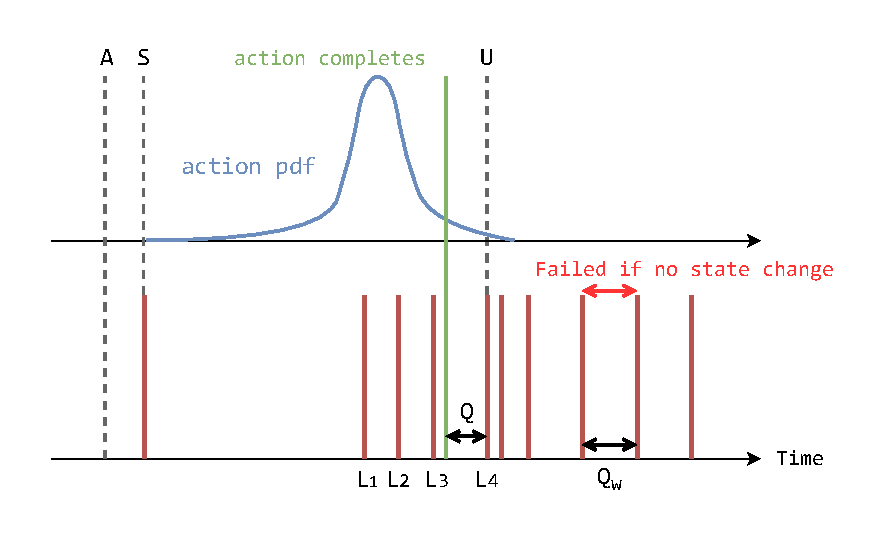
\includegraphics[width=0.7\linewidth,alt={Poll-placement example for RASC with k equal to 4. Red lines are RASC polls issued after the action starts; the action completes between the third and fourth poll. The action is expected to complete between the first and second poll with much higher probability following a bell curve, and the polling interval is larger for the end of the action, where the action truly completes. If the action never made progress after the fourth poll, it would be detected after exponential increase in polling interval up to $Q_w$.}]{RASC/figures/design/rasc.pdf}
    \caption{\bf \small Placement Example, $k = 4$. {\it Red lines are \abstraction{}  polls (after action start). Action completes between third and fourth poll.}}
    \medskip
    \label{rasc:fig:poll}
\end{figure}


\noindent \textbf{Reducing Polling further via  Confidence Intervals.} 
We relax the worst-case detection time assumption by introducing a {\it service-level objective (SLO)}: a confidence level for meeting the detection window $Q_w$. 
When SLO=0.9, \sysname's placement may violate $Q_w$ on at most 10\% of events. 
This allows \sysname{} to avoid excessive polling in high probability areas of the distribution.
Our evaluations (\Cref{rasc:sec:detection_times}) find that  SLO-awareness does not change average detection time. \Cref{rasc:algo:adaptive-polling-algorithm} shows how to find polls under SLOs.

\begin{theorem}[Meeting a Detection Tolerance SLO--Condensed version]
Given a detection window $Q_w \in (0, U]$, a service-level objective (SLO) $\text{slo}\in(0,1]$, and a placement
$\mathcal{L}=\{L_1<\dots<L_k=U\}$, its covered set is
\[
C(\mathcal{L})=\bigcup_{i=1}^{k}\big((L_i-Q_w)^+,\,L_i\big]\cap(0,U],
\quad (x)^+=\max\{x,0\},
\]
and its coverage is
\[
\mathrm{Cover}(\mathcal{L})=\int_{C(\mathcal{L})}\!p(t)\,dt.
\]
Let $A_k(Q_w)$ denote the best achievable coverage with $k$ polls,
\[
\begin{aligned}
A_k(Q_w) &= \max_{\mathcal{L}}\, \mathrm{Cover}(\mathcal{L}),\\
k^*(\text{slo},Q_w) &= \min\{\,k\in\mathbb{N}: A_k(Q_w)\ge \text{slo}\,\}.
\end{aligned}
\]
Assume a binary search over $k$ is run with initial bracket $\texttt{left}=0$, $\texttt{right}=\lceil U/Q_w\rceil$,
using an oracle \texttt{examineQw} that returns \texttt{true} exactly when there exists a placement $\mathcal{L}$ with $\mathrm{Cover}(\mathcal{L})\ge \text{slo}$.
Then the search returns $k^*(\text{slo},Q_w)$ together with an $\text{slo}$-feasible placement.
\end{theorem}

\begin{proof}
\noindent\textbf{Monotonicity.} If $k'<k$, any $k'$-poll placement can be extended to $k$ polls by inserting additional polls; this cannot reduce $C(\mathcal{L})$, hence $A_k(Q_w)\ge A_{k'}(Q_w)$. The oracle predicate is therefore nondecreasing in $k$.

\noindent\textbf{Bracketing.} For $k=\lceil U/Q_w\rceil$, equal spacing $L_i=iU/k$ yields $\bigcup_i ((L_i-Q_w)^+,L_i]\supseteq(0,U]$, so $\mathrm{Cover}(\mathcal{L})=1\ge \text{slo}$. Thus the upper bracket is feasible, while $k=0$ is not.

\noindent\textbf{Minimality via binary search.} Binary search on a non-decreasing predicate with a feasible upper bracket returns the smallest $k$ for which the predicate holds; by definition, this is $k^*(\text{slo},Q_w)$.
\end{proof}

\subsubsection{Detection Beyond  Upper Bound}
\label{rasc:sec:detect-after-U}

Upper bound estimates for action completion may be violated due to 
human interference (e.g., propped elevator doors), environmental factors (e.g., 
colder weather slowing a heater), and out-of-order requests (e.g., the elevator moving from 1st to 3rd floor receives a 2nd-floor request). 
Consequently,
if no state change occurs by time $U$, polling must continue. 
The key question is: {\it 
What is the optimal post-$U$ polling technique?} 

Our key observation is that past $U$, the chance of an imminent state change typically declines, so \sysname{} polls densely before tapering. 
We distinguish actions by progress:
for those showing {\it some} partial progress (e.g., vacuum location changed), we estimate the remaining time via the observed rate (time to the current progress) and schedule the next poll at $min\{\text{estimate}, Q_w\}$. Otherwise, \sysname{} uses \textit{exponential backoff}, doubling the inter-poll gap up to $Q_w$, to avoid overloading troubled devices while ensuring detection within $Q_w$ (\Cref{rasc:fig:poll}).
If no change occurs within $Q_w$ {after the upper bound $U$} 
we declare the action failed. In our experiments, overruns beyond $U$ are rare, and late actions typically finish soon after $U$. 
